\def\documentType{Protocol}
\def\mainLanguage{ngerman}

\input{template.tex}

\pgfqkeys{/TemplateVersion0}{
    properties/Authors 				= {Tom Mohr&&Martin Ohmeyer},
    properties/Title	 			= {Versuch V7},
    properties/Subtitle 			= {C405 Hardwarepraktikum II},
    properties/Institution 			= {HTWK Leipzig},
    properties/Group 				= {23INB-3},
    properties/Versioning 	      	= {true},
    misc/Date/Prefix				= {Stand: },
    misc/Page/CountPrefix			= {Seiten: },
    misc/Group/Prefix				= {Gruppe: },
    Protocol/Comment		 	    = {Abnahme: 06. Januar 2025}
}

%\usepackage{minted}
%\usepackage{subcaption}
%\usepackage{siunitx}
\usepackage{tikz}
\usepackage[table]{xcolor}
\usepackage[utf8]{inputenc}
\usepackage{color,soul}
\usepackage{mathtools}
\usepackage{transparent}
\usepackage{adjustbox}
\usepackage{tcolorbox}
\usepackage{inconsolata}
\usetikzlibrary{decorations.pathreplacing}
\usetikzlibrary{arrows, automata, positioning}
\graphicspath{{../images/}}

\begin{document}

    \chapter{Einleitung}
Im Nachfolgenden finden Sie unser Versuchsprotokoll zu V7. Es beleuchtet nur unseren finalen, erfolgreichen Ansatz. Was es nicht beinhaltet, sind die insgesamt vier gescheiterten Ansätze über einen Zeitraum von mehr als 2 Monaten, welche uns bis hierher gebracht haben. Während der Bearbeitung des Versuches mussten wir auf Basis neuer Erkenntnisse ständig nachjustieren und ganze Programme verwerfen. Die Kodierung hat sich von einer fixen Escape-Sequenz zur jetzigen dynamischen entwickelt, die Threadaufteilung wurde mehrmals verworfen und die Modularisierung des Programms hat fortlaufend zugenommen. Nun sind wir an einem Punkt, an dem unser Programm mit jeder Hardware funktioniert, welche die Methoden \texttt{send()} und \texttt{receive()} unseres Kommunikations-Interfaces in C++ implementieren kann. Unsere Anwendung setzt sich in ihrer finalen Version aus über 25 Klassen und vielen ungebunden Funktionen zusammen. Optimierungspotential gibt es sicherlich noch immer, aber wie es eben in der Informatik so ist, muss man sich irgendwann mit einer Lösung abfinden, welche gut genug ist.

\vspace{1cm}
\noindent
Unseren gesamten Quelltext finden Sie im Git-Repository unter dem folgendem Link.
\begin{tcolorbox}[colback=gray!10,colframe=black,boxrule=0.5pt]
\href{https://github.com/tomo2403/HTWK-C405-HWP2.git}{https://github.com/tomo2403/HTWK-C405-HWP2.git}
\end{tcolorbox}
\vspace{0.5cm}

\noindent
Bitte beachten Sie, dass einige Bezeichner hier im Protokoll vereinfacht und/oder übersetzt wurden. Viele Klassen wurden zur simpleren Funktionserläuterung des Programms wegabstrahiert. Dieses Protokoll soll einen groben Überblick über unsere Software geben und sie nicht ausgiebig dokumentieren. Sie finden alle erwähnten Konzepte und Module des Protokolls im Code wieder, dies aber vielleicht unter anderem Namen oder in noch mehr Module aufgespalten, als hier gezeigt.
    \chapter{Kodierung}
\section{Notwendigkeit}
\label{sec:notwendigkeit}
Nacheinander gesendete Nibble müssen auf der Leitung voneinander unterscheidbar sein. Um dies zu gewährleisten, wird ein Taktsignal in den Datenstrom kodiert, indem verhindert wird, dass ein gesendetes Nibble gleich seinem Vorgänger ist. Dies verursacht den Sonderfall zweier gleicher aufeinanderfolgender Nibble. Zu dessen Behandlung muss eine Escape-Sequenz definiert werden, welche die gleichen Nibble durchbricht. Durch die Einführung einer solchen Escape-Sequenz wird ihr eigenes Auftreten im Datenstrom jedoch selbst zu einem Sonderfall. Zur Handhabung dieser Sonderfälle und zur Definition von Blöcken wurde ein Protokoll zwischen Sender und Empfänger vereinbart.

\section{Besondere Sequenzen}
Aus den in \ref{sec:notwendigkeit} dargelegten Gründen werden vordefinierte Sequenzen in den Datenstrom injiziert. Eine solche Sequenz setzt sich aus vier festen (Escape-Sequenz) und vier dynamischen Bits (Handlungsanweisung: "Command") zusammen.

\begin{figure}[H]
    \centering
    \[
        \underbrace{\text{XXXX}}_\text{\normalsize esc} \ \overbrace{\text{XXXX}}^\text{\normalsize cmd}
    \]
    \caption{Aufbau einer Kodierungssequenz}
\end{figure}

Die \textbf{Escape-Sequenz} trennt kodierende Sequenzen vom restlichen Datenstrom ab. Sie selbst hält keine Information darüber, um welche Kodierung es sich handelt. Aufgrund ihrer Sonderfunktion darf sie nicht regulär im Datenstrom auftreten und muss ggf. selbst escaped werden.

\textbf{Commands} erhalten erst dann ihre Bedeutung, wenn sie unmittelbar nach der Escape-Sequenz stehen. Sie geben Auskunft darüber, um welche Kodierung es sich handelt und implizieren, wie sich ein Dekodierender verhalten muss, um die originalen Daten wieder zu rekonstruieren. Ist das nachfolgende Nibble auf einen Command (im binären) mit diesem identisch, wird anstelle des normalen Commands dessen Fallback-Version genutzt.

\begin{table}[H]
    \center
    \def\arraystretch{1.3}
    \rowcolors{2}{gray!15}{white}
    \begin{tabular}{|c|l|l|l|}
        \rowcolor{gray!50}
        \hline
        \textbf{Hex} & \textbf{Bezeichnung}          & \textbf{Bedeutung}                 \\
        \hline
        0            & escapeSequence                & Das nächste Nibble ist ein Command \\
        1            & beginDataBlockDefault         & Ein Datenblock beginnt             \\
        2            & beginDataBlockFallback        & Ein Datenblock beginnt             \\
        3            & beginControlBlockDefault      & Ein Kontrollblock beginnt          \\
        4            & beginControlBlockFallback     & Ein Kontrollblock beginnt          \\
        5            & endBlockDefault               & Der aktuelle Block endet           \\
        a            & endBlockFallback              & Der aktuelle Block endet           \\
        6            & insertPrevNibbleAgainDefault  & Ein doppeltes Nibble im Datenstrom \\
        7            & insertPrevNibbleAgainFallback & Ein doppeltes Nibble im Datenstrom \\
        8            & insertEscSeqAsDataDefault     & Die Esc-Seq trat im Datenstrom auf \\
        9            & insertEscSeqAsDataFallback    & Die Esc-Seq trat im Datenstrom auf \\
        \hline
    \end{tabular}
    \caption{Bitsequenzen und ihre Bedeutung}
    \label{tab:escape_sequences}
\end{table}

\section{Datenblöcke}
    \chapter{Implementation}
\section{Parallelisierung}
Zeitmessungen des Schreib- und Lesezugriffs auf das B15 Board haben ergeben, dass diese Vorgänge jeweils 15,8ms - 16,2ms dauern. Da wir eine Voll-Duplex Kommunikation erreichen sollen, müssen wir beides im Wechsel tun. Ein Leseaufruf kann also im schnellsten Fall ca. alle 32ms erfolgen.

Das Abarbeiten eingehender Nibble dauert unterschiedlich lang, abhängig davon an welcher Stelle, des zugehörigen Datenpakets, sich das Nibble befindet. 4 Bit in der Mitte eines Pakets werden einfach an einen Vektor hinten angehängt und sind abgearbeitet, während das letzte Nibble der End-Sequenz einen umfangreichen Validierungsprozess des gesamten aktuellen Pakets anstößt. Diese unterschiedlichen Bearbeitungszeiten erschweren ein präzises Timen der Lese- und Schreibzugriffe auf die Hardware. Als Konsequenz scheiterte ein früherer Single-Thread-Ansatz daran, dass einzelne Nibble in unregelmäßigen Abständen vom B15 Board überlesen wurden. Daher ist es notwendig, die verarbeitende Logik und die Hardwarezugriffe voneinander zu trennen. Dies wir durch das Aufspalten jener Vorgänge in separate Threads erreicht. Ein vereinfachtes Modell der Threads ist in Abbildung \ref{fig:datenfluss} dargestellt.

Das Grundkonzept ist eine mini Pipeline, in welcher jeder Thread, dank zwischengeschalteter Warschlangen, unabhängig von der Geschwindigkeit aller anderen Threads operieren kann. Der Hardwarethread ist dadurch der Lage in jedem Fall alle vordefinierten $n$ Sekunden zu lesen und zu schreiben. Die Wartezeit zwischen jedem Zyklus kann präzise mittels Delay eingestellt werden, ohne dass die Berechnungszeit anderer Vorgänge abfälschend einwirkt.

\begin{figure}[H]
    \centering
    \begin{adjustbox}{scale=0.6}
        \input{../images/multithread.pdf_tex}
    \end{adjustbox}
    \caption{Datenfluss innerhalb eines Kommunikationsteilnehmers (abstrakt)}
    \label{fig:datenfluss}
\end{figure}

\section{Der Sender}
Der Sender ist das Herzstück des Programms. Er verfügt von Haus aus über die Information, wie weit er mit dem Sendefortschritt ist und wann ein Paket vollständig auf die Leitung gebracht wurde. Folglich ist er auch für Timeout-Erkennung nach dem Versand zuständig. Die Funktionalität des Senders wurde als Zustandsautomat modelliert und implementiert. Die Verbildlichung dieses Automaten ist in der folgenden Darstellung \ref{fig:zustandsautomat} zu sehen. Zustandswechsel werden durch interne Ereignisse (z.B. Datenpaket gesendet) oder externe Informationen aus dem Empfänger (z.B. Neusenden eines Paketes erforderlich) ausgelöst.

\vspace{0.5cm}
\begin{figure}[H]
    \centering
    \label{fig:zustandsautomat}
    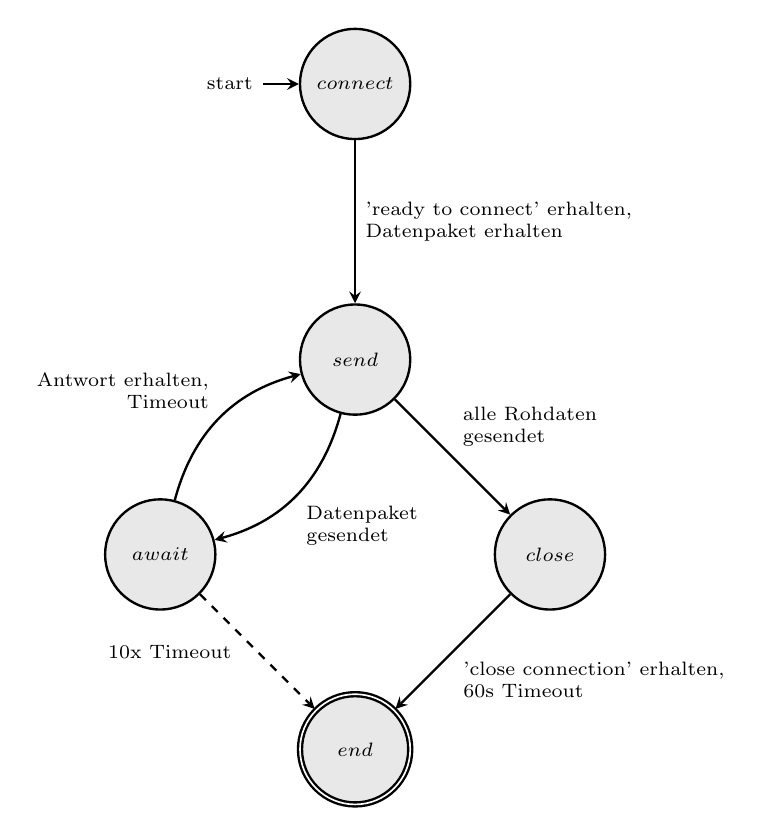
\begin{tikzpicture} [on grid, auto, node distance=3.5cm]
        \tikzstyle{every state}=[fill={rgb:black,1;white,10}, minimum size=1.4cm]
        \tikzstyle{every path}=[>=stealth, line width=0.3mm]
        \tikzset{font=\scriptsize}

        \node[state,initial]    (ready)                                 {$connect$};
        \node[state]            (sending)   [below of=ready]            {$send$};
        \node[state]            (awaiting)  [below left of=sending]     {$await$};
        \node[state]            (close)     [below right of=sending]    {$close$};
        \node[state, accepting] (end)       [below right of=awaiting]   {$end$};

        \path[->]
        (ready)     edge            node[align=left]                    {'ready to connect' erhalten,\\Datenpaket erhalten}  (sending)
        (sending)   edge[bend left] node[align=left]                    {Datenpaket\\gesendet}                               (awaiting)
        (awaiting)  edge[bend left] node[align=right]                   {Antwort erhalten,\\Timeout}                         (sending)
        (sending)   edge            node[align=left]                   {alle Rohdaten\\gesendet}                            (close)
        (close)     edge            node[align=left]                   {'close connection' erhalten,\\60s Timeout}          (end)
        (awaiting)  edge[dashed]    node[left,align=left,xshift=-0.2cm] {10x Timeout}                                        (end);

    \end{tikzpicture}
    \vspace{0.5cm}
    \caption{Zustandsautomat des Senders}
\end{figure}
\vspace{1cm}
\noindent

\noindent
Im \textbf{Connect-Zustand} wird in 3s Intervallen ein 'ready to connect'-Kontrollpaket auf die Leitung gesendet. Wird ein solches Paket, oder ein Datenpaket, empfangen findet ein Wechsel in den nächsten Zustand statt.
Im \textbf{send-Zustand} wird dann ein Datenpaket gesendet. Ist sein Versand abgeschlossen, wird in den \textbf{await-Zustand} gewechselt und auf eine Antwort des Kommunikationspartners gewartet. Entweder diese wird erhalten, oder es kommt noch 30s zu einem Timeout. Wurde bereits 10 Mal ohne erhaltene Rückmeldung versucht ein Paket zu senden, wird eine Timeout-Exception ausgelöst und das Programm kontrolliert zum Absturz gebracht. Sonst geht es zurück in den send-Zustand, wo entweder das nächste oder erneut das vorherige Paket gesendet wird, je nach Verhalten des Kommunikationspartners. Wurden alle Rohdaten gesendet, kann die Verbindung geschlossen werden. Dafür wird in den \textbf{close-Zustand} gewechselt. In diesem werden keine neuen Daten mehr gesendet und nur noch auf eingehende Pakete geantwortet. Zusätzlich wird dem Kommunikationspartner in 3s Intervallen mitgeteilt, dass alle Daten gesendet wurden und die Verbindung geschlossen werden kann. Gibt auch der Kommunikationspartner diese Meldung zurück, terminiert das Programm. Sollten die 'close connection'-Kontrollpakete verloren gehen, schließt sich die Verbindung nach 60s ohne neuem eingehenden Nibble selbstständig.


\section{Der Empfänger}
Der Empfänger hat deutlich weniger komplexe Logik als der Sender und kommt ohne Zustandsautomat aus. Seine Hauptaufgabe im Versand- und Empfangsprozess ist das Auswerten erhaltender Daten- und Kontrollblöcke und das Informieren des Senders. Dafür nutzt der Empfänger eine threadsichere Nachrichtenwarteschlange, über welche er dem Sender Informationen zukommen lassen kann. Die Nutzung dieses Nachrichtensystems ist in Abbildung \ref{fig:datenfluss} durch den pinken Pfeil angedeutet. Nach Erhalt eines Datenpaketes veranlasst dort der Empfänger den Sender dazu, eine Antwort an den Kommunikationspartner zu schicken. Eine Auflistung der Benachrichtigungen erfolgt in Tabelle \ref{tab:benachrichtigungen}.

\begin{table}[H]
    \center
    \def\arraystretch{1.3}
    \rowcolors{2}{gray!15}{white}
    \begin{tabular}{|l|l|}
        \rowcolor{gray!50}
        \hline
        \textbf{Bezeichnung}  & \textbf{Bedeutung}                                      \\
        \hline
        startSendingData      & 'ready to connect'-Paket empfangen; Kom.-Partner online \\
        closeConnection       & 'close connection'-Paket empfangen; Kom.-Partner fertig \\
        foreignPacketResend   & Fordere Neusenden eines Paktes von Kom.-Partner         \\
        foreignPacketReceived & Bestätige Kom.-Partner  Paketerhalt                     \\
        ownPacketResend       & Kom.-Partner fordert Neusenden eines Pakets             \\
        ownPacketReceived     & Kom.-Partner bestätigt Paketerhalt                      \\
        \hline
    \end{tabular}
    \caption{Interthreadbeanchrichtigungen}
    \label{tab:benachrichtigungen}
\end{table}
    

\chapter{Geschwindigkeit}
\section{B15 zu Arduino}
In der Kommunikation zwischen B15 Board und Arduino ist ersteres der Flaschenhals. Mit einer maximalen Schreib- und Lesegeschwindigkeit von einem Nibble in 32ms im Best-Case, ist mit viel Glück eine Geschwindigkeit von 15,625 B/s das erreichbare Maximum der rohen Übertragungsgeschwindigkeit. Bei Praxistests dieser Werte, ist durch das Schwanken der Antwortzeiten des B15-Interfaces die Übertragung jedoch instabil und fehlerlastgig geworden. Zur Kompensation musste ein Lese-/Schreibzyklus auf 35ms erhöht werden, was nur noch eine rohe Geschwindigkeit von 14,285 B/s erlaubt. Dazu kommt Overhead durch das Mitsenden von Start- und Endsequenzen, dem CRC, einer Paket-ID und vor allem der Übermittlung von Antworten. All dies berücksichtigt, übertragen wir nun mit ca. 10.5 B/s die tatsächlichen Nutzdaten. Als Erwähnung sei hinzugefügt: Bei Tests mit 2 Arduinos haben wir Geschwindigkeiten von ca. 1200 kB/s bei der Nutzdatenübertragung erreicht.

\section{netcat}
Auf der Senderseite werden die Rohdaten mit folgenden Befehl in netcat gepiped und die Übertragungsziet gestoppt.
\begin{tcolorbox}[colback=gray!10,colframe=black,boxrule=0.5pt]
\begin{verbatim}
time cat input_file | nc -q 0 141.57.56.143 20000
\end{verbatim}
\end{tcolorbox}

\noindent
Die Empfängerseite lässt sich über folgenden Befehl starten.

\begin{tcolorbox}[colback=gray!10,colframe=black,boxrule=0.5pt]
\begin{verbatim}
nc -q 0 -l -p 20000 > received_file
\end{verbatim}
\end{tcolorbox}

\noindent
Dabei haben wir für eine 10.671.180B große Datei 3.054s benötigt. Das entspricht einer Übertragungsgeschwindigkeit von 3,49 MB/s.

\newpage

\section{scp}
Zum Zeitmessen des Sendens einer Datei mittels scp haben wir einen SSH-Key auf dem Zielrechner hinterlegt, um die Messung nicht durch eine menschliche Passworteingabe zu verfälschen. Mit folgendem Command wurde die Datei im Anschluss auf ada3 hochgeladen.

\begin{tcolorbox}[colback=gray!10,colframe=black,boxrule=0.5pt]
\begin{verbatim}
scp input_file mohmeyer@142.57.6.153:/home/mohmeyer
\end{verbatim}
\end{tcolorbox}

\noindent
Die erreichte Geschwindigkeit wurde nach der Übertragung von scp direkt selbst angezeigt und lag bei 19,1MB/s.

\end{document}